\documentclass[10pt]{beamer}

\usetheme[progressbar=frametitle]{metropolis}
\usepackage{appendixnumberbeamer}
\usepackage{booktabs}
\usepackage[scale=2]{ccicons}
\usepackage{pgfplots}
\usepgfplotslibrary{dateplot}
\usepackage{mathtools}
\DeclarePairedDelimiter{\ceil}{\lceil}{\rceil}
\usepackage{xspace}
\usepackage{amsmath}
\newcommand{\themename}{\textbf{\textsc{metropolis}}\xspace}

\usefonttheme{professionalfonts} % using non standard fonts for beamer
\usefonttheme{serif} % default family is serif

\usepackage{tipa}
\usepackage{xcolor}

\definecolor{myBlue}{HTML}{7982db}
\definecolor{myGreen}{HTML}{ABDDA4}
\definecolor{myBlue2}{HTML}{4169AA}
\definecolor{myGreen2}{HTML}{38AE40}

\usetikzlibrary{arrows} % For arrows :"D



% For Arabic
\usepackage{polyglossia} 
\setmainlanguage{english}
\setotherlanguage{arabic}
% Defining the font family
\newfontfamily\arabicfont  [Script=Arabic, Scale=1.5]{Scheherazade}%
\newfontfamily\arabicfontsf[Script=Arabic, Scale=1.5]{Scheherazade}%

\usepackage{bidipoem}

\title{Learning Meters of Arabic and English poems}
\subtitle{With Recurrent Neural Networks}
\date{\today}
\author{
Prof. Waleed A. YOUSEF \\
The Team}
\institute{Computer Science department\\
Faulty of Computers and Information, Helwan University}

%\title{A Practical Introduction to Natural Language Processing}
%
%\subtitle{Intelligent Processing \& Applications\\Research Cluster Seminar}
%
%%\date{5 \& 12 March 2015}
%%\date{5 March 2015\\Session 1: Common Tasks and Concepts in NLP}
%%\date{12 March 2015\\Session 2: Software Libraries and Resources for NLP}
%\date{5 March 2015\\Session 1: Common Tasks and Concepts in NLP\\[0.5ex]
%12 March 2015\\Session 2: Software Libraries and Resources for NLP}
%\author{Dr Lim Lian Tze}
%\institute{
%Information Technology Department\\
%School of Science, Engineering and Technology\\
%KDU College Penang
%}

\begin{document}
\setbeamertemplate{caption}{\raggedright\insertcaption\par}


\maketitle

\begin{frame}{Table of contents}
  \setbeamertemplate{section in toc}[sections numbered]
  \tableofcontents[hideallsubsections]
\end{frame}



% 1
\section{Introduction}
\begin{frame}[fragile]{Hello, Arabic}
    \begin{center}
    \begin{Arabic}
    ودعْ عنك آراءَ الرجالِ وقولَهم\hspace{3em}  فقولُ رسولِ الله أزكى وأشرحُ
    \end{Arabic}
    \end{center}
\end{frame}


% But ... What is poetry?
\begin{frame}[fragile]{But ... What is poetry?}

\textbf{\large General Definition}:
\begin{itemize}
  \item \textbf{Poetry} is a piece of writing or speaking, which
\textbf{\textcolor{red}{MUST}} follow specific
\alert{\underline{\textbf{Patterns}}}.
\end{itemize}

\vspace{0.5cm}
\textbf{\large Example}, \textit{\small English verse}:
\begin{center}
That 
  \textcolor{myGreen2}{\textbf{time}} of 
  \textcolor{myGreen2}{\textbf{year}} thou
  \textcolor{myGreen2}{\textbf{mayst}}  in 
  \textcolor{myGreen2}{\textbf{me}}
be\textcolor{myGreen2}{\textbf{hold}}
\end{center}

To detect poems' meters, we need to learn those \alert{\textbf{Patterns}}.
\end{frame}




\begin{frame}[fragile]{Arabic Prosody \textarabic{العَرُوض}}

\begin{itemize}
  \item \textbf{Foot} \textarabic{التفعيلة}: is a sequence of vowels and consonants.
\end{itemize}




\begin{center}
  \begin{tabular}{|c|c|} \hline
    \textbf{Feet} & \textbf{Scansion} \\
    \hline
    \textarabic{فَعُولُنْ}  & \texttt{0/0//}\\
    \textarabic{فَاعِلُنْ}  & \texttt{0//0/}\\
    \textarabic{مُسْتَفْعِلُنْ}& \texttt{0//0/0/}\\
    \textarabic{مَفاعِيلُنْ}& \texttt{0/0/0//}\\
    \textarabic{مَفْعُولاَت} & \texttt{0//0///}\\
    \textarabic{فَاعِلاَتُنْ} & \texttt{0/0//0/}\\
    \textarabic{مُفَاعَلَتُنْ}& \texttt{0///0//}\\
    \textarabic{مُتَفَاعِلُنْ}& \texttt{0//0///}\\
    \hline
  \end{tabular}
\end{center}

\end{frame}





\begin{frame}[fragile]{Arabic Prosody \textarabic{العَرُوض}}

Arabic Patterns/Meters \textarabic{بحور الشعر}:
\begin{itemize}
  \item \textbf{Meter} \textarabic{البحر}: is a sequence of \alert{feet}. 
\end{itemize}

\begin{center}
  \begin{tabular}[h!]{|c|c|} 
    \hline
    \textbf{Meter Name} & \textbf{Meter} \small{\textit{feet combination}} \\ 
    \hline
   \textit{al-Wafeer}    & \textarabic{مُفَاعَلَتُن مُفَاعَلَتُن فَعُولُن} \\ %
   \textit{al-Taweel}    & \textarabic{فَعُوْلُنْ مَفَاْعِيْلُنْ فَعُوْلُنْ مَفَاْعِلُنْ} \\ %
   \vdots                &  \vdots\\
   \textit{al-Moktadib}  & \textarabic{مَفْعُوْلاتُ مُسْتَفْعِلُنْ مُسْتَفْعِلُن} \\
   \textit{al-Modar'e}   & \textarabic{مَفَاْعِيْلُنْ فَاْعِلاتُنْ مَفَاْعِيْلُنْ} \\
    \hline
  \end{tabular}
\end{center}

\end{frame}




\begin{frame}[fragile]{Arabic Prosody, example!}

\textbf{From \textarabic{بحر الوافر}}:
\begin{center}
  \textarabic{ويسْأل فىْ الْحواْدث ذوْ صواْبٍ}\\
  \textarabic{ويسأل فل \hspace{0.4cm}
    حوادث ذو\hspace{0.4cm}
    صوابن}\\
  \texttt{0/0//     \hspace{0.3cm}
          0///0//   \hspace{0.3cm}
          0///0//}\\

  \textarabic{مفاْعلتنْ\hspace{0.7cm} 
    مفاْعلتنْ          \hspace{0.7cm}
    فعوْلنْ}
\end{center}

\end{frame}





\begin{frame}[fragile]{English Prosody}


\textbf{English Meters Building Blocks}:
\begin{itemize}
  \item Syllables: \textipa{\sffamily /"wO:t@/} = \textipa{\sffamily /"wO:/}  $+$ \textipa{\sffamily /t@(r)/}.
    \begin{itemize}
         \item \textcolor{myGreen2}{\textbf{stressed}} $+$ unstressed.
    \end{itemize}
  \item Foot: is a combination of stressed and unstressed syllables. 

\end{itemize}

\begin{center}
\begin{tabular}{|c | c|} 
    \hline
    %\toprule
    Feet     & Stresses Combination\\ 
    \hline
    %\toprule
    \textit{Iamb} & $\times$\textit{/}\\             %\midrule
    \textit{Trochee}& \textit{/}$\times$\\           %\midrule
    \textit{Dactyl} & \textit{/}$\times\times$\\     %\midrule
    \textit{Anapest}& $\times\times$\textit{/}\\     %\midrule
    \textit{Pyrrhic}& $\times\times$\\               %\midrule
    \textit{Amphibrach}& $\times$\textit{/}$\times$\\%\midrule
    \textit{Spondee}& \textit{/}\textit{/}\\
    %\bottomrule
    \hline
\end{tabular}
\end{center}

\textbf{Meter}: is repeating a foot $n$ times; where $n \in [1, 8]$. 
\end{frame}





\begin{frame}[fragile]{English Patterns}

Iambic pentameter verse:
\begin{center}
$\underbrace{\text{That \textcolor{myGreen2}{\textbf{time}}}
}_\text{Iambic Foot}$\hspace{0.2cm}
%
$\overbrace{\text{of \textcolor{myGreen2}{\textbf{year}}}
}^\text{2nd}$\hspace{0.2cm}
%
$\overbrace{\text{thou \textcolor{myGreen2}{\textbf{mayst}}}
}^\text{3rd}$\hspace{0.2cm}
%
$\overbrace{\text{in \textcolor{myGreen2}{\textbf{me}}}
}^\text{4th}$\hspace{0.2cm}
%
$\overbrace{\text{be\textcolor{myGreen2}{\textbf{hold}}.}
}^\text{5th}$\hspace{0.2cm}
\end{center}
\end{frame}






% Literature 
\section{Literature Review}
\begin{frame}[fragile]{Detecting Arabic poems' Meters}

\textbf{Abuata and Al-Omari}:
    \begin{itemize}
        \item Five-step Algorithm
            \begin{enumerate}
                \item Getting the input, carrying full diacritics.
                \item Metrical scansion rules are applied to the Arud writing. 0/0/..
                \item Grouping zero and ones to feet \textarabic{تفعيلات}.
                \item A class is assigned  to the input.
            \end{enumerate}
        \item \textbf{\alert{Results}}: 82.2\% of 417 verses.
    \end{itemize}
\textbf{Alnagdawi et al}, similar approach;  Context-Free Grammar; 75\% correctly
classed from 128.
\end{frame}

\begin{frame}[fragile]{example!}

\begin{center}
  \textarabic{ويسْأل فىْ الْحواْدث ذوْ صواْبٍ}\\
  \textarabic{ويسأل فل \hspace{0.4cm}
    حوادث ذو\hspace{0.4cm}
    صوابن}\\
  \texttt{0/0//     \hspace{0.3cm}
          0///0//   \hspace{0.3cm}
          0///0//}\\

  \textarabic{مفاْعلتنْ\hspace{0.7cm} 
    مفاْعلتنْ          \hspace{0.7cm}
    فعوْلنْ}
\end{center}

\end{frame}

\begin{frame}[fragile]{Abuata and Al-Omari \&\& Alnagdawi et al; Problems}
Issues;
    \begin{itemize}
       \item A huge constrain. \alert{Diacritics} are a must.
        % A source of randomness.
       \item Converting the text into pronounced text is \alert{probabilistic}.
            \begin{itemize}
                % الرحمن لكن هذا إله السموات
                \item \textarabic{اثبات الحروف المحذوفة خطاً}
                \item \textarabic{التصرف فى التقاء الساكنين}
            \end{itemize}
    \end{itemize}
\end{frame}




\begin{frame}[fragile]{Tanasescu et al.}
Binary Classification; Metric or Free-Verse: 
        \begin{itemize}
            \item verses are represented as vectors of statistical features.
        \end{itemize}
\end{frame}


\section{Datasets}
\begin{frame}[fragile]{Datasets}
\textbf{Arabic Dataset}:
\begin{center}
\begin{tikzpicture}[scale=0.75]
\begin{axis}[
    symbolic x coords={Taweel,
   Kamel,
   Baseet,
   Khafeef,
   Wafeer,
   Rigz,
   Raml,
   Motakarib,
   Sar'e,
   Monsafeh,
   Mogtath,
   Madeed,
   Hazg,
   Motadarik,
   Moktadib,
   Modar'e
    },
    xtick=data,
    % the following x label positioning does work here.
    every axis y label/.style= {at={( 0.1, 1.1)}, anchor=north},
    %ylabel style={font=\footnotesize},
    xticklabel style = {font=\footnotesize},
    ylabel={Class size},
    x=0.4cm,
    x tick label style={rotate=60, anchor=east}, 
    % Y ticks configurations
    y tick label style={/pgf/number format/.cd,%
      scaled y ticks = false,
      set thousands separator={,},
      fixed},]
    \addplot[ybar,fill=myBlue] coordinates {
        (Taweel, 416428)
        (Kamel,  370116)
        (Baseet, 244583)
        (Khafeef,     157880)
        (Wafeer,     143148)
        (Rigz,     119286)
        (Raml,     79560)
        (Motakarib,     63613)
        (Sar'e,     59370)
        (Monsafeh,     28768)
        (Mogtath,     18062)
        (Madeed,     7808)
        (Hazg,     7468)
        (Motadarik,     5144)
        (Moktadib,     799 )
        (Modar'e,     288 )
    };
\end{axis}
\end{tikzpicture}

\end{center}
\end{frame}

\begin{frame}[fragile]{Datasets}
\textbf{English Dataset}:
\begin{center}
\begin{tikzpicture}[scale=0.8]
\begin{axis}[
    symbolic x coords={
   Iambic,
   Trochaic,
   Anapaestic,
   Dactyl,
    },
    xtick=data,
    % the following x label positioning does work here.
    every axis y label/.style= {at={( 0.1, 1.1)}, anchor=north},
    %ylabel style={font=\footnotesize},
    xticklabel style = {font=\footnotesize},
    ylabel={Class size},
    x=1.7cm,
    /pgf/bar width=15pt,
    x tick label style={rotate=60, anchor=east}, 
    % Y ticks configurations
    y tick label style={/pgf/number format/.cd,%
      scaled y ticks = false,
      set thousands separator={,},
      fixed},]
    \addplot[ybar,fill=myBlue] coordinates {
        (Iambic, 5550)
        (Trochaic,  5422)
        (Anapaestic, 5380)
        (Dactyl,     1397)
    };
\end{axis}
\end{tikzpicture}

\end{center}
\end{frame}


\section{Methodology}
\begin{frame}[fragile]{Which Network!}


\begin{columns}


\begin{column}{0.7\textwidth}
\begin{itemize}
    \item[--] \textbf{Pattern}: is a sequance of characters.
    \item  Unlike feedforward neural networks, RNNs can use their internal state (memory) to process sequences of inputs.
\end{itemize}

\end{column}



\begin{column}{0.5\textwidth}  %%<--- here
    \begin{figure}
        \begin{center}
         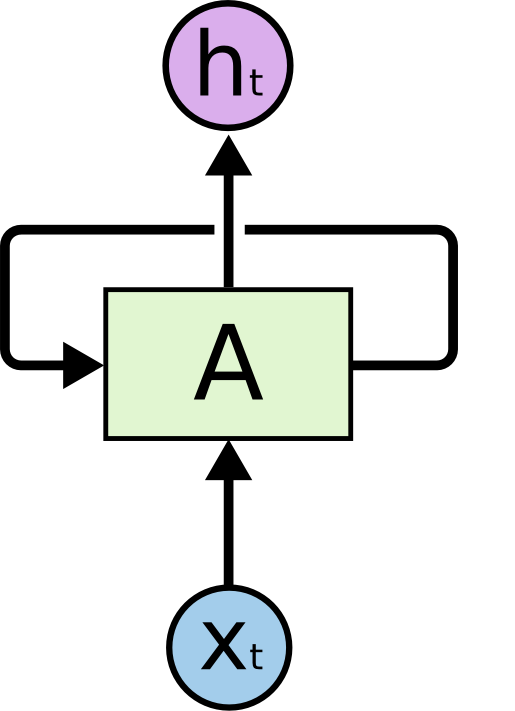
\includegraphics[width=0.5\textwidth]{rolledRNN.png}
         \caption{Rolled Rnn unit}
         \end{center}
    \end{figure}
\end{column}
\end{columns}
\end{frame}



\begin{frame}[fragile]{RNN, Architectures}

\begin{center}
    \begin{tikzpicture}
%\draw[step=0.5, gray, very thin] (0,0) grid (10, 7);

\def \sRight {0}

\node[inner sep=0pt] (russell) at (5 +\sRight, 5)
    {\includegraphics[width=.30\textwidth]{LSTM.png}};

\node[inner sep=0pt] (russell) at (5 +\sRight, 2)
    {\includegraphics[width=.33\textwidth]{GRU.png}};

\node[inner sep=0pt] (russell) at (9.7 +\sRight, 4)
    {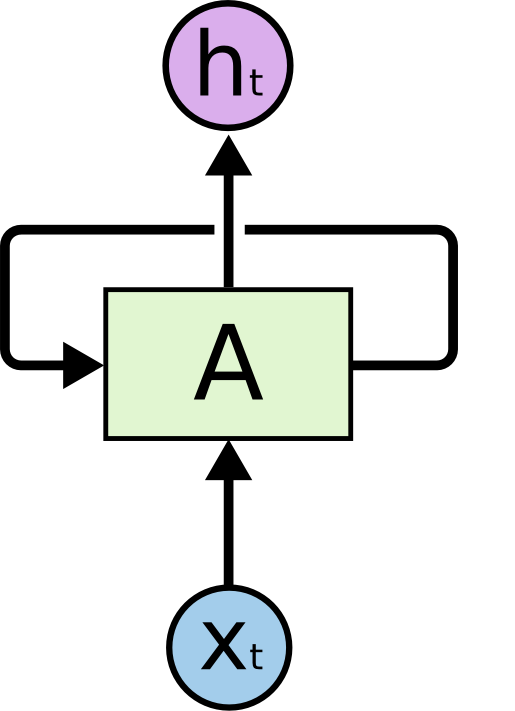
\includegraphics[width=.30\textwidth]{rolledRNN.png}};

\draw[arrows=-angle 90, line width=2pt, myBlue2]  (8.5, 3.7) -- (6.5, 4.75);
\draw[arrows=-angle 90, line width=2pt, myBlue2]  (8.5, 3.5) -- (6.5, 1.75);


\node at (3, 4.4) {\tiny  $h_{t - 1}$};
\node at (3, 5.4) {\tiny  $C_{t - 1}$};

\node at (6.8, 4.4) {\tiny  $h_{t}$};
\node at (6.8, 5.4) {\tiny  $C_{t}$};
%\node[draw,text width=9cm] at (0, 6) {
%   \begin{minipage}{9cm}
%    \small
%        \begin{align*}
%          f_t  &= \sigma(W_f  x_t + U_f h_{t-1} + b_t)\\
%          i_t  &= \sigma(W_i  x_t + U_i h_{t-1} + b_i)\\
%          o_t  &= \sigma(W_o  x_t + U_o h_{t-1} + b_o)\\
%          C_t  &= f_t \circ c_{t-1} + i_t \circ tanh(W_c x_t + U_c h_{t-1} + b_c)\\
%          h_t  &= o_t \circ tanh(c_t)
%        \end{align*}
%    \end{minipage}
%};


\node at (2.3, 5) {LSTM unit};
\node at (2.3, 1.8) {GRU unit};
\end{tikzpicture}


\end{center}
\begin{itemize}
    \item Two variants of unidirectional \textit{recurrent units}.
\end{itemize}
\end{frame}

\begin{frame}[fragile]{RNN, Architectures}
Bi-direction unit.
\end{frame}

\begin{frame}[fragile]{Data Representation}
An Issue:
\begin{itemize}
    \item Diacritics are standalone characters!
    \begin{itemize}
        \item \texttt{len} \textarabic{مرحبا} $\neq$ \texttt{len} \textarabic{مَرْحَبَاً}
        \item We have represented the letter and its diacritic as a \alert{one
character}.
    \end{itemize}
\end{itemize}
\textbf{Benefits}:
\begin{enumerate}
    \item Verse's length is fixed, regardless the diacritic states.
    \item Saving more space, by shorten the length of full diacritic verses. 
    \item Models can be tested on both diacritic or non-diacritic data.
\end{enumerate}
\end{frame}

\begin{frame}[fragile]{Encoding Techniques}
\begin{enumerate}
    \item One-Hot
    \item Binary
    \item \alert{Two-Hot} (new technique)

\end{enumerate}
\end{frame}

\begin{frame}[fragile]{One-Hot}
    \begin{center}
        \begin{tikzpicture}
% helper grid
%    \draw[step=0.5, gray, very thin] (0,0) grid (4,5);

\node at (2, 0) {\textit{One-Hot Vector}: from $37 \times 1$ to $181 \times 1$};

% Change lengths to change the rec hieght 
% [DO NOT play with the coordinates].
\def \recLengthFirst   {2.5}
\def \recLengthSecond  {3}
\def \recWidth         {0.5}

%% Positioning rectangles.
% Stating point of the First rectangle
\def \xF {0} % right and left
\def \yF {1} % up and down
% Stating point of the Second rectangle
\def \xS {3} % right and left
\def \yS {0.75} % up and down

% First Rectangle (on the right)
\draw[rounded corners=1pt] (\xF, \yF) 
    rectangle (\recWidth, \yF + \recLengthFirst)
         node [above, xshift=-0.25cm] {\textarabic{ب}};

% Second Rectangle (on the left)
\draw[rounded corners=1pt] (\xS, \yS) 
    rectangle (\xS + \recWidth, \yS + \recLengthSecond) 
        node [above, xshift=-0.25cm] {\textarabic{ب}};


% The coordinate of the rectangle's top y .
\def \topF {\recLengthFirst + \yF}
% Populating the first rectangle.
\newcommand\numbers{{0.25, 0.6, 0.95, 1.3, 1.65, 2, 2.35, 2.7}}
\node at (0.25, \topF - \numbers[0]) {0};
\node at (0.25, \topF - \numbers[1]) {1};
\node at (0.25, \topF - \numbers[2]) {0};
\node at (0.25, \topF - \numbers[3]) {\vdots};
\node at (0.25, \yF + \numbers[1])   {0};
\node at (0.25, \yF + \numbers[0])   {0};

% Annotating the first rectangle.
\def \leftDistance {-0.4}
\draw[arrows=->] (\leftDistance, \yF + 1.59) -- (\leftDistance, \yF + 2.4);
\draw[arrows=<-] (\leftDistance, \yF + 0.1) -- (\leftDistance, \yF + .94);

% Transformation  Arrow
\def \arrowY {\yF + \recLengthFirst/2}
\draw[arrows=-angle 90, line width=2pt] (1, \arrowY) -- (2.5, \arrowY);
\node at (\leftDistance, \arrowY) {37};

% Annotating the first rectangle.
\def \rightDistance {0.4}
\draw[arrows=->] (\rightDistance +3.5, \yF + 1.59) -- (\rightDistance +3.5, \yF + 2.67);
\draw[arrows=<-] (\rightDistance +3.5, \yF - 0.2 ) --  (\rightDistance +3.5, \yF + .94);
\node at (\rightDistance + 3.5, \arrowY) {181};



%  Populating 
\def \topS {\recLengthSecond + \yS}
\node at (\xS + .25, \topS - \numbers[0]) {0};
\node at (\xS + .25, \topS - \numbers[1]) {1};
\node at (\xS + .25, \topS - \numbers[2]) {0};
\node at (\xS + .25, \topS - 1.4)         {\vdots};
\node at (\xS + .25, \yS + \numbers[2])   {0};
\node at (\xS + .25, \yS + \numbers[1])   {0};
\node at (\xS + .25, \yS + \numbers[0])   {0};



\end{tikzpicture}

    \end{center}
181 is the number of all combination between letters and diacritics.\\
$181 = 36 + 36 \times 4 + 1$
\end{frame}

\begin{frame}[fragile]{One-Hot, example}
    \begin{center}
        \begin{tikzpicture}   
% Rectangles
% the space between each rectangular
\def \x {0.57} 
\def \s {1} % I'll use it to shift to right
% A list of letters <3
\newcommand\letters{{"ا","بَ","حَ", "رْ", "مَ"}}

% Rectangle
\def \length {2.95}
\foreach \j in {0,...,4} 
    \draw [rounded corners=1pt] (\s+\x*\j, 0) rectangle (\s+0.5+\x*\j, \length) 
    node[above, xshift=-0.25cm]
    {\textarabic{\pgfmathparse{\letters[\j]}\pgfmathresult}};

% Above Annotation
% Cell line
% 0.25*10+0.09 = 2.59
\def \d {3.9 - 0.15}
\draw (\s+0.25-0.007, 3.9 ) -- (\s+2.53+0.007, 3.9 ); % the main bar
\draw (\s+0.25, 3.9 ) -- (\s+0.25, \d ); % sub bar #ا
\draw (\s+0.25*3+0.03, 3.9 ) -- (\s+0.25*3+0.03, \d ); % sub bar #ب
\draw (\s+0.25*5+0.15, 3.9+0.15 ) -- (\s+0.25*5+0.15, \d ) 
    node[above, yshift=0.3cm]{\textarabic{مَرْحَبَا}}; % sub bar #ح
\draw (\s+0.25*7+0.2, 3.9 ) -- (\s+0.25*7+0.2, \d ); % sub bar #ر
\draw (\s+2.53, 3.9 )  -- (\s+2.53, \d );  % sub-bar #م

% adding numbers, vector ا
\node at (\s+0.25, \length - 0.25)    {1}; % the top number; using -
\node at (\s+0.25, \length - 0.6)     {0};
\node at (\s+0.25, \length - 0.95)    {0};
\node at (\s+0.25, \length - 1.3)     {0};
\node at (\s+0.25,  1.1)     {\vdots};
%\node at (\s+0.25, \length - 1.65)    {0};
%\node at (\s+0.25, \length - 2)       {0};
%\node at (\s+0.25, \length - 2.35)    {0};
\node at (\s+0.25, \length - 2.7)     {0};

% distance between vectors elements
\def \d {0.07}
% adding numbers, vector ب
\node at (\s+0.25*3+\d, \length - 0.25)    {0}; % the top number; using -
\node at (\s+0.25*3+\d, \length - 0.6)     {\vdots};
%\node at (\s+0.25*3+\d, \length - 0.95)    {0};
\node at (\s+0.25*3+\d, \length - 1.18)     {1};
\node at (\s+0.25*3+\d, 1.28) {\vdots};
\node at (\s+0.25*3+\d, \length - 2.35)    {0};
\node at (\s+0.25*3+\d, 0.25) {0}; % The bottom  number


% adding numbers, vector ح
\node at (\s+0.25*5+\d*2, \length - 0.25)    {0}; % the top number; using -
\node at (\s+0.25*5+\d*2, \length - 0.6)     {\vdots};
\node at (\s+0.25*5+\d*2, \length - 1.35)     {1};
\node at (\s+0.25*5+\d*2, 1.18) {\vdots};
\node at (\s+0.25*5+\d*2, \length - 2.35)    {0};
\node at (\s+0.25*5+\d*2, 0.25) {0}; % The bottom  number

% adding numbers, vector ر
\node at (\s+0.25*7+\d*3, \length - 0.25)    {0}; % the top number; using -
\node at (\s+0.25*7+\d*3, \length - 0.6)     {0};
\node at (\s+0.25*7+\d*3, \length - 0.95)     {0};
\node at (\s+0.25*7+\d*3, \length - 1.33)     {\vdots};
\node at (\s+0.25*7+\d*3, 1.07) {1};
\node at (\s+0.25*7+\d*3, \length - 2.2)    {\vdots};
\node at (\s+0.25*7+\d*3, 0.25) {0}; % The bottom  number

% adding numbers, vector م
\node at (\s+0.25*9+\d*4, 3 - 0.25) {0}; % the top number; using -
\node at (\s+0.25*9+\d*4, 3 - 0.69) {0};
\node at (\s+0.25*9+\d*4, 0.25) {0};
\node at (\s+0.25*9+\d*4, 0.25*4 - 0.1) {\vdots};
\node at (\s+0.25*9+\d*4, 0.9 + 0.4) {1};
\node at (\s+0.25*9+\d*4, 1.3 + 0.6) {\vdots};

% Vector size annotations.
% figures starts at x = 1
\def \d {0.6} % Annotation x=0.4
\draw[arrows=->] (\d, 1.7) -- (\d, 2.9); % up-line
\draw[arrows=<-] (\d, 0.1) -- (\d, 1.1) node[above, yshift=0.07cm]
{{\textcolor{red}{\small{181}}}};
% bottom-line

\draw[arrows=<-] (\s+0.1, -0.4) -- (\s+1.19, -0.4) node[right, xshift=0.05cm] {\small{5}};
\draw[arrows=->] (\s+1.2+0.5, -0.4) -- ( \s+2.7,-0.4);

\end{tikzpicture}%

    \end{center}
\end{frame}

\begin{frame}[fragile]{Binary}
Let $n$ be the vector length.\\
$n = \ceil*{\log_2 l}$ $l \in \{181, 28\}$
    \begin{center}
        \begin{tikzpicture}[x=1cm,y=1cm]

% Rectangles
% the space between each rectangular
\def \x {0.57} 
\def \s {1} % I'll use it to shift to right
% A list of letters <3
\newcommand\letters{{"ا","بَ","حَ", "رْ", "مَ"}}

%\draw[step=0.2, gray, very thin, red] (1,-0.5) grid (4,4);

% Rectangulars
\def \length {2.95}
\foreach \j in {0,...,4} 
    \draw[rounded corners=1pt] (\s+\x*\j, 0) rectangle (\s+0.5+\x*\j, \length) 
    node[above, xshift=-0.25cm]
    {\textarabic{\pgfmathparse{\letters[\j]}\pgfmathresult}};

% Above Annotatios
% Cell line
% 0.25*10+0.09 = 2.59
\def \d {3.9 - 0.15}
\def \z {0.2}
\draw (\s+0.25-0.007, 3.9 ) -- (\s+2.53+0.007, 3.9 ); % the main bar
\draw (\s+0.25, 3.9 ) -- (\s+0.25, \d ); % sub bar #ا
\draw (\s+0.25*3+0.03, 3.9 ) -- (\s+0.25*3+0.03, \d ); % sub bar #ب
\draw (\s+0.25*5+0.15, 3.9+0.15 ) -- (\s+0.25*5+0.15, \d ) 
    node[above, yshift=0.3cm]{\textarabic{مَرْحَبَا}}; % sub bar #ح
\draw (\s+0.25*7+0.2, 3.9 ) -- (\s+0.25*7+0.2, \d ); % sub bar #ر
\draw (\s+2.53, 3.9 )  -- (\s+2.53, \d );  % sub-bar #م

% adding numbers, vector ا
\node at (\s+0.25, \length - 0.25)    {0}; % the top number; using -
\node at (\s+0.25, \length - 0.6)     {0};
\node at (\s+0.25, \length - 0.95)    {0};
\node at (\s+0.25, \length - 1.3)     {0};
\node at (\s+0.25, \length - 1.65)    {0};
\node at (\s+0.25, \length - 2)       {0};
\node at (\s+0.25, \length - 2.35)    {0};
\node at (\s+0.25, \length - 2.7)     {1};

% distance between vectors elements
\def \d {0.07}
% adding numbers, vector ب
\node at (\s+0.25*3+\d*1, \length - 0.25)    {0}; % the top number; using -
\node at (\s+0.25*3+\d*1, \length - 0.6)     {0};
\node at (\s+0.25*3+\d*1, \length - 0.95)    {1};
\node at (\s+0.25*3+\d*1, \length - 1.3)     {0};
\node at (\s+0.25*3+\d*1, \length - 1.65)    {0};
\node at (\s+0.25*3+\d*1, \length - 2)       {1};
\node at (\s+0.25*3+\d*1, \length - 2.35)    {1};
\node at (\s+0.25*3+\d*1, \length - 2.7)     {1};


% adding numbers, vector ح
\node at (\s+0.25*5+\d*2, \length - 0.25)    {0}; % the top number; using -
\node at (\s+0.25*5+\d*2, \length - 0.6)     {0};
\node at (\s+0.25*5+\d*2, \length - 0.95)    {1};
\node at (\s+0.25*5+\d*2, \length - 1.3)     {0};
\node at (\s+0.25*5+\d*2, \length - 1.65)    {1};
\node at (\s+0.25*5+\d*2, \length - 2)       {0};
\node at (\s+0.25*5+\d*2, \length - 2.35)    {1};
\node at (\s+0.25*5+\d*2, \length - 2.7)     {1};

% adding numbers, vector ر
\node at (\s+0.25*7+\d*3, \length - 0.25)    {1}; % the top number; using -
\node at (\s+0.25*7+\d*3, \length - 0.6)     {0};
\node at (\s+0.25*7+\d*3, \length - 0.95)    {0};
\node at (\s+0.25*7+\d*3, \length - 1.3)     {1};
\node at (\s+0.25*7+\d*3, \length - 1.65)    {1};
\node at (\s+0.25*7+\d*3, \length - 2)       {0};
\node at (\s+0.25*7+\d*3, \length - 2.35)    {1};
\node at (\s+0.25*7+\d*3, \length - 2.7)     {1};

% adding numbers, vector م
\node at (\s+0.25*9+\d*4, \length - 0.25)    {0}; % the top number; using -
\node at (\s+0.25*9+\d*4, \length - 0.6)     {0};
\node at (\s+0.25*9+\d*4, \length - 0.95)    {1};
\node at (\s+0.25*9+\d*4, \length - 1.3)     {1};
\node at (\s+0.25*9+\d*4, \length - 1.65)    {1};
\node at (\s+0.25*9+\d*4, \length - 2)       {1};
\node at (\s+0.25*9+\d*4, \length - 2.35)    {0};
\node at (\s+0.25*9+\d*4, \length - 2.7)     {1};

% Vector size annotations.
% figures starts at x = 1
\def \vColumn {0.6} % Annotation x=0.4
\draw[arrows=->] (\vColumn, 1.7) -- (\vColumn, 2.9); % up-line
\draw[arrows=<-] (\vColumn, 0.1) -- (\vColumn, 1.1) node[above, yshift=0.07cm] {\textcolor{red}{\small{8}}};
% bottom-line

\draw[arrows=<-] (\s+0.1, -0.4) -- (\s+1.19, -0.4) node[right, xshift=0.05cm] {\small{5}};
\draw[arrows=->] (\s+1.2+0.5, -0.4) -- ( \s+2.7,-0.4);


\end{tikzpicture}

    \end{center}
\end{frame}

\begin{frame}[fragile]{Two-Hot}
    \begin{center}
        \begin{tikzpicture}[scale=0.9]
\small
% The grid
%\draw[step=0.5, gray!40, very thin] (0,0) grid (6,4);

\def \recWidthA {0.5}
\def \yStartA   {1.5}
\def \yEndA     {3}
\def \xStartA   {1.5}
\def \xEndA     {0.5}
\def \xStartB   {0}
\def \yStartB   {1}
\def \xEndB     {2}
\def \yEndB     {3.5}
\def \half      {\yEndA/2 - \yStartA/2}
\def \xStartC   {3 +0.5}
\def \yStartC   {0.5 -.1}
\def \xEndC     {3.5 +0.5}
\def \yEndC     {4 +.1 }
\def \shiftMargin {0.3}
\newcommand\numbers{{0.25, 0.6, 0.95, 1.3, 1.65, 2, 2.35, 2.7}}

% Rectangle A
\draw[rounded corners=2pt] (\xStartA, \yStartA) rectangle (\xStartA + \recWidthA, \yEndA)
node [above, xshift=-.25cm] {\textarabic{◌َ}};
% Populating the rectangle A
\node at (0.25 + \xStartA, 3 -\numbers[0]) {1};
\foreach \j in {1,...,3}
    \node at (0.25 + \xStartA, \yEndA -\numbers[\j]) {0};



% Rectangle B
\draw[rounded corners=2pt] (\xStartB +0.5, \yStartB) rectangle (\yStartB +0.5 -1.5, \yEndB)
node[above, xshift=0.25cm] {\textarabic{ب}};
\node at (\xStartB +0.25, \yEndB -\numbers[0]) {0};
\node at (\xStartB +0.25, \yEndB -\numbers[1]) {1};
\node at (\xStartB +0.25, \yEndB -\numbers[2]) {0};
\node at (\xStartB +0.25, \yEndB -\numbers[3]) {0};
\node at (\xStartB +0.25, \yEndB -\numbers[4] ) {\vdots};
\node at (\xStartB +0.25, \yStartB +\numbers[0]) {0};

% Annotation B
\node at (-\shiftMargin, \yStartA + \half) {\small 37};
\draw[arrows=-angle 90, very thin] (-\shiftMargin, \yStartA + \half +.3) -- (-\shiftMargin, \yEndB -0.1);
\draw[arrows=angle 90-, very thin] (-\shiftMargin, \yStartB + .1) -- (-\shiftMargin, \yStartA + \half -.3);




\node at (1, \yStartA +\half) {$+$};
\node at (2.5 + .02, \yStartA +\half) {$=$};

% Rectangle C
\draw[rounded corners=2pt]  (\xStartC, \yStartC) rectangle (\xEndC, \yEndC)
node[above, xshift=-0.25cm] {\textarabic{بَ}};
;
\node at (\xStartC +0.25, \yEndC -\numbers[0]) {1};
\node at (\xStartC +0.25, \yEndC -\numbers[1]) {0};
\node at (\xStartC +0.25, \yEndC -\numbers[2]) {0};
\node at (\xStartC +0.25, \yEndC -\numbers[3]) {0};

\node at (\xStartC +0.25, \yEndC -\numbers[4] -.2) {0};
\node at (\xStartC +0.25, \yEndC -\numbers[5] -.2) {1};
\node at (\xStartC +0.25, \yEndC -\numbers[6] -.2) {0};
\node at (\xStartC +0.25, \yEndC -\numbers[7] -.2) {\vdots};
\node at (\xStartC +0.25, \yStartC +\numbers[0]) {0};

% Annotation
\node at (\xStartC -\shiftMargin, \yStartA +\half) {\small 41};
\draw[arrows=-angle 90, very thin]  (\xStartC -\shiftMargin, 2.5) -- (\xStartC -\shiftMargin, \yEndC -0.1);
\draw[arrows=angle 90-, very thin]  (\xStartC -\shiftMargin, 0.5) -- (\xStartC -\shiftMargin, 2);

\draw [decorate,decoration={brace,amplitude=2pt,mirror,raise=2pt}, very thin]
    (\xEndC +\shiftMargin -.1, 2.5 +.2) -- (\xEndC +\shiftMargin  -.1, \yEndC -0.1) 
    node [right, midway, xshift=0.2cm, yshift=0.1cm] {\small $4 \times 1$ diacritic vector};

\draw [decorate,decoration={brace,amplitude=2pt,mirror,raise=2pt}, very thin]
    (\xEndC +\shiftMargin -.1, 0.5) -- (\xEndC +\shiftMargin -.1, 2.4)
    node [right, midway, xshift=0.2cm, yshift=0.1cm] {\small $37 \times 1$ letter vector};

\node at (5.6 + 0.5, 3.2 - 0.1) {\small which represents \textarabic{◌َ}};
\node at (5.5 + 0.5, 1.3 - 0.1) {\small which represents \textarabic{بَ}};


\node at (0.25, 0.5) {$m$};
\node at (1.5 +.25, 0.5 +0.5) {$k$};

\end{tikzpicture}

    \end{center}
\end{frame}



\begin{frame}[fragile]{Space Comparison}
    \begin{center}
        \begin{tikzpicture}[scale=0.9]
\begin{axis}[
    symbolic x coords={
    % the x ordering.
    One-Hot,
    Two-Hot,
    Binary,
    },
    xtick=data,
    % the following x label positioning does work here.
    every axis y label/.style= {at={( 0.1, 1.1)}, anchor=north},
    ylabel={Bytes},
    x=2cm,
    ytick={7216, 35632, 161728},
    % X ticks configurations
    x tick label style={anchor=north},
    % Y ticks configurations
    y tick label style={/pgf/number format/.cd,%
      scaled y ticks = false,
      set thousands separator={,},
      fixed},] 

    \addplot[ybar,fill=myBlue] coordinates {
        % Ordering does not effect.
        (One-Hot, 161728)
        (Two-Hot, 35632)
        (Binary,  7216)
    };
\end{axis}
\end{tikzpicture}

    \end{center}
\end{frame}

%\begin{frame}[fragile]{Arabic Patterns}
%ello
%\end{frame}










\section{Results}  









\end{document}
